\documentclass [12pt]{article}
\usepackage{epsfig}
\usepackage{enumitem}
\usepackage{amsmath}
% \usepackage[color, leftbars]{changebar}
% \usepackage{fontawesome} 
% \usepackage{caption}
% \usepackage{subcaption}


\setlength{\textwidth}{6.5in}
\setlength{\textheight}{9in}
\setlength{\oddsidemargin}{0in}
\setlength{\evensidemargin}{0in}
\setlength{\topmargin}{-0.5in}

\setlength{\parindent}{0pt}

% \newtheorem{theorem}{Theorem}[section]
% \newtheorem{definition}[theorem]{Definition}
% \newtheorem{claim}[theorem]{Claim}
% \newtheorem{lemma}[theorem]{Lemma}
% \newtheorem{proof}[theorem]{Proof}

\newlength{\toppush}
\setlength{\toppush}{2\headheight}
\addtolength{\toppush}{\headsep}

\usepackage{hyperref}
\hypersetup{
    colorlinks=true,
    linkcolor=blue, % was previously black
    filecolor=magenta,
    urlcolor=blue,
    pdftitle={Template}
}
\urlstyle{same}


\def\subjnum{EE 156}
\def\subjname{Adv. Comp. Arch.}

\def\doheading#1#2#3{\vfill\eject\vspace*{-\toppush}%
  \vbox{\hbox to\textwidth{{\bf} \subjnum: \subjname \hfil Amy Bui}%
    \hbox to\textwidth{{\bf} Tufts University, Spring 2023 \hfil#3\strut}%
    \hrule}}

\newcommand{\htitle}[1]{\vspace*{3.25ex plus 1ex minus .2ex}%
\begin{center}
{\large\bf #1}
\end{center}} 

%%%%%%%%%%%%%%%%%%%%%%%%%%%%%%%%%%%%%%%%%%%%%%%%%%%%%%%%%%%%%%%%%%%

\begin{document}
\doheading{2}{title}{Noise Notes and PR} 
% \htitle{Paper Info}
% \bigskip 
% \bigskip 
%%%%%%%%%% begin text after this line %%%%%%%%%%%%%%

    \section{Necessity of Noise Modeling} %%%
        \begin{itemize}
            \item A quantum system has to involve some incoherence processes (measurements, random perturbations, etc), which ultimately makes the system probabilistic. So a noisy quantum system produces a random distribution of quantum states $| \psi_{i} \rangle$ with probability $p_{i}$ due to imprecise controls and environmental noise \cite{ding}.
            
            \item Start by modeling noise as a probability distribution over pure quantum states, $\{ p_i, | \psi_i \rangle \}$ \cite{ding}.
            
            \item Noise is pervasive, difficult to characterize/understand, and can have multiple sources, but you cannot consider practical quantum computing without considerations for effects of noise on the quantum system. 
            
            
            \item Noise modeling informs how noise disrupts correctness during computation. The better they are, the better research can facilitate simulations, because actual quantum computers are few and far between. 
            
            \item Determining specific noise requires physical experiments, which is not feasible for most users. Realistic noise models are not feasible to simulate at scale, so noise is estimated and these simulation techniques make simplifying assumptions.  
            
            \item quantum noise is context dependent, so estimating error for one gate does not necessarily model larger systems with more qubits. Qubit errors cannot be considered independently. This makes noise impossible to simulate. This impacts benchmarking quantum computers, as error rates may increase with larger systems due  to increase complexity (i.e. extrapolating information from running a program on small system does not straightforwardly inform how it runs on a larger system).
        \end{itemize}

    %%%%%%%%%%%%%%%%%%%%%%%%%%%%%%%%%%%%%%%%%%%%%%%%%%%%%%%

    \section{Basic of Noise Characterization}
        \begin{itemize}
            \item Different errors that noise can introduce (leading to the different noise models) \cite{resch21}:
                \begin{itemize}

                    \item undesired \textbf{environment} interactions or decay of quantum states
                        \begin{itemize}
                            \item Ideal scenario is complete isolation from environment, which is not possible, so the goal is increased coherence time. 
                            \item Measured with: coherence time, dephasing time, and relaxation time
                            \item Performing operations on a quantum system requires external input to the system, so this also increases risk of environmental interactions (coherence-controllability tradeoff). 
                            \item these interactions can also lead to unitary errors that cause unitary rotation of quantum states
                        \end{itemize}

                    \item undesired \textbf{qubit qubit} interactions
                        \begin{itemize}
                            \item qubits can become entangled and their states correlated. Entanglement is only useful when users desire it. 
                            \item Unexpected entanglement of qubits lead to mixture of quantum states and decoherence/degredation of quantum state (cross-talk), when what we actually want to happen with cross-talk is just a unitary evolution of the state in order to retain information in the quantum state rather than losing the information. 
                            \item Ancilla (extra) qubit interactions (with data qubit) is a technique used for error correction, where error information (syndromes) is extracted by measuring ancilla. However, this itself can lead to cross-talk between ancilla and data qubit, where data qubit loses quantum information to the ancilla and its state is changed.
                        \end{itemize}
                    
                    \item imprecise \textbf{control} of operations 
                        \begin{itemize}
                            \item perfect application of gates gives us precise correct quantum states; 
                            \item imperfect calibrations lead to slightly different rotations, which doesn't directly destroy quantum states but rather evolves it to an unwanted state. This affects the ability of error correction techniques.  
                        \end{itemize}
                    
                    \item \textbf{Leakage} to other quantum states:
                        \begin{itemize}
                            \item Computation works on the assumption that qubits are encoded in \textbf{computational subspace}, where only two possible states are represented ($| 0 \rangle$ \emph{or} $| 1 \rangle$).
                            \item quantum systems that we use as qubits actually have more states than that. 
                            \item Leakage: when a qubit enters one of the other states outside of subspace. 
                            \item Seepage: when a qubit returns to computational subspace. 
                            \item Leakage and seepage can be caused by one of the other error sources. 
                        \end{itemize}
                \end{itemize}

            \item 
        \end{itemize}

    %%%%%%%%%%%%%%%%%%%%%%%%%%%%%%%%%%%%%%%%%%%%%%%%%%%%%%%

    \section{Some Noise Models}
        \begin{itemize}
            \item Stochastic Pauli Noise 
                \begin{itemize}
                    \item Simple and easy to correct for \cite{wallman16}
                    \item models undesired environment interactions
                    \item SPN is implemented by inserting a X, Y, or Z gate into a circuit at random. Certain error rates for each gives us depolarizing noise or symmetric depolarizing noise. 
                    \item SPN can be considered inaccurate and overly optimistic, can provide reasonable approximations of certain conditions \cite{resch21}
                    \item Improving on SPN can involve augmenting Pauli gates with Clifford group operators (H, S, and CNOT) and Pauli measurements (i.e. simply using a larger set of gates for the random insertion)
                \end{itemize}

            \item Coherent Noise 
            \item Amplitude/Phase Damping 
            \item Overview of which physical noise can correspond to which noise model \cite{resch21}: 
            
                \begin{center}
                    \begin{tabular}{p{5cm}|p{7cm}}
                        \hline 
                        Physical Noise Source & Noise Model \\ 
                        \hline 
                        \hline
                        Environment Interaction & Stochastic Pauli Noise, Amplitude/Phase Damping, Pauli Measurements \\ 
                        \hline
                        Imperfect Control & Coherent Over/Under Rotations \\ 
                        \hline
                    \end{tabular}
                \end{center}
        \end{itemize}



    \section{Reference Formulas and Definitions} %%%
        \begin{itemize}
            \item Coherence time: time that a quantum system can stay undisturbed (i.e. isolated from interactions with environment)
            
            \item Qubit relaxation time: time it takes for loss of energy from system. 
            
            \item Dephasing time: time it takes to polarize qubit that is in superposition (i.e. from $| 0 \rangle$ \emph{and} $| 1 \rangle$, to $| 0 \rangle$ \emph{or} $| 1 \rangle$)
            
            \item coherence-controllability tradeoff: the conflicting requirements for quantum computation are quantum states needing isolation to remain intact and quantum states must have interactions with control mechanisms in order to yield useful computation \cite{resch21}
            
            \item Cross-talk: unexpecteed qubit-qubit interaction (entanglement) that mixes their states and leads to decoherence. 
            
            \item Quantum Circuit Model: For an $n$-qubit quantum system,
            $$ | \psi \rangle = \sum_{b\in\{0,1\}^n} \alpha_b | b \rangle $$
            Coefficient $\alpha_b$ is the amplitude of basis bit-string $b$. 

            \item The joint state of two separate quantum systems is represented with \emph{tensor product}, $| \psi_0 \rangle \otimes | \psi_1 \rangle$
            
            \item trace of a matrix is the sum of its diagonal elements, i.e. diagonal sum. $|e_i\rangle$  is the basis vector with 1 at the $i^{\text(th)}$ index, and 0 everywhere else: $$ \textbf{tr}(A) = \sum_i A_{ii} = \sum_i | e_i \rangle A | e_i \rangle  $$
            
            \item density matrix representation, $\rho$, is how mixed state is represented: $$ \rho = \sum_i p_i | \psi_i \rangle | \psi_i \rangle $$
            
            \item trace and density matrix helps define the fidelity metric for quantifying the quality of a quantum state: $ \textbf{tr}(\rho \sigma)  $, where $\sigma$ is actual quantum state, versus the density matrix or ``correct'' quantum state \cite{resch21}.
            
            \item Unitary coupling transformation $U$ represents the impact on noise/the environment on a quantum state. $U$ is applied to both environment and syste, $\rho_{\text{env}} \otimes \rho_{\text{in}}$
            
                \begin{figure}[htb!]
                    \centering
                    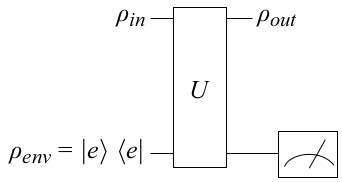
\includegraphics[width=0.25\textwidth]{images/unitaryCouplingTransformation.png}
                \end{figure}

            \item linear map: $\rho \rightarrow \mathcal{E}(\rho)$
            \item The unitary operator: $ \mathcal{E}(\rho) = U \rho U^{\dag} $
            \item operator form for entire unitary coupling evolution, with environment, $U$, and measurement. $U$ acts on both system and environment.  
                $$ \rho_{\text{in}} \rightarrow \rho_{\text{out}} = \textbf{tr}_{\text{env}}(U (\rho_{\text{env}} \otimes \rho_{\text{in}}) U^{\dag}) $$
        \end{itemize}
    %%%%%%%%%%%%%%%%%%%%%%%%%%%%%%%%%%%%%%%%%%%%%%%%%%%%%%%


    \section{Paper Overviews} %%%

    \begin{itemize}
        \item Salonik Resch and Ulya R. Karpuzcu. 2021. \href{https://dl-acm-org.ezproxy.library.tufts.edu/doi/10.1145/3464420}{Benchmarking Quantum Computers and the Impact of Quantum Noise}. ACM Comput. Surv. 54, 7, Article 142 (September 2022), 35 pages.
            \begin{itemize}
                \item Details benchmarking quantum computers from a computer architecture perspective and the challenges, as well as the significance and complexity of things that have to be considered when benchmarking, such as noise model (and ability to simulate and/or characterize), target application, and performance metrics. The authors categorize some physical noise sources (environment or other qubits), and overviews some noise models (Stochastic Pauli Noise, Coherent Noise, Amplitude/Phase Damping) and references other related works that cover these models. They also go over different metrics and how different ones may be preferred (process fidelity, average gate fidelity/infidelity, trace distance, Hellinger fidelity). They run benchmarks on a few quantum benchmarks and use the process fidelity metric to illustrate the impact of noise.
            \end{itemize}

        \item M. A. Nielsen and I. L. Chuang, Quantum Computation and Quantum Information (Cambridge University Press, Cambridge, 2012). Chapter 9.
            \begin{itemize}
                \item (classical) Fidelity is defined as the distance between probability distributions, $p$ and $q$: 
                
                $$ F(p_x, q_x) = \sum_x \sqrt{p_x q_x} $$

                \item Trace Distance for two quantum states: 
                $$  D(\rho, \sigma) = \frac{1}{2}\textbf{tr}|\rho - \sigma| $$

                \item (quantum) Fidelity of two states: 
                $$  F(\rho, \sigma) = \textbf{tr} \sqrt{\sqrt{\rho} \sigma \sqrt{\rho}} $$
            \end{itemize}

    \end{itemize}

    %%%%%%%%%%%%%%%%%%%%%%%%%%%%%%%%%%%%%%%%%%%%%%%%%%%%%%%%%%%%%%%%





\begin{thebibliography}{1}
    \bibitem[ding2020]{ding}Y. Ding, F. Chong. \href{https://link.springer.com/book/10.1007/978-3-031-01765-0}{Quantum Computer Systems: Research for Noisy Intermediate-Scale Quantum Computers}. Springer Cham. Synthesis Lectures on Computer Architecture. 2020

    \bibitem[resch21]{resch21}Salonik Resch and Ulya R. Karpuzcu. 2021. \href{https://dl-acm-org.ezproxy.library.tufts.edu/doi/10.1145/3464420}{Benchmarking Quantum Computers and the Impact of Quantum Noise}. ACM Comput. Surv. 54, 7, Article 142 (September 2022), 35 pages.

    \bibitem[barnes17]{barnes17}Barnes, Jeff P. and Trout, Colin J. and Lucarelli, Dennis and Clader, B. D.\href{https://arxiv.org/abs/1704.03961}{Quantum error-correction failure distributions: Comparison of coherent and stochastic error models}. American Physical Society. Phys. Rev. A, Vol.. 95, Issue 6 (June 2017).

    \bibitem[beale18]{beale18}Stefanie J. Beale, Joel J. Wallman, Mauricio Gutiérrez, Kenneth R. Brown, and Raymond Laflamme. 2018. \href{https://link.aps.org/accepted/10.1103/PhysRevLett.121.190501}{Quantum
    error correction decoheres noise}. Phys. Rev. Lett. 121, 19 (2018), 190501.

    \bibitem[bravyi18]{bravyi18}Sergey Bravyi, Matthias Englbrecht, Robert König, and Nolan Peard. 2018. \href{https://www.nature.com/articles/s41534-018-0106-y}{Correcting coherent errors with surface
    codes}. npj Quant. Inf. 4, 1 (2018), 55.

    \bibitem[duckering2020]{duckering2020}C. Duckering, J. M. Baker, D. I. Schuster and F. T. Chong, "\href{https://ieeexplore-ieee-org.ezproxy.library.tufts.edu/document/9251988}{Virtualized Logical Qubits: A 2.5D Architecture for Error-Corrected Quantum Computing}," 2020 53rd Annual IEEE/ACM International Symposium on Microarchitecture (MICRO), Athens, Greece, 2020, pp. 173-185, doi: 10.1109/MICRO50266.2020.00026.

    \bibitem[wallman15]{wallman15}Joel Wallman, Chris Granade, Robin Harper, and Steven T. Flammia. 2015. Estimating the coherence of noise. New J. Phys. 17, 11 (2015), 113020.

    \bibitem[nickerson19]{nickerson19}Naomi H. Nickerson and Benjamin J. Brown. 2019. \href{https://arxiv.org/abs/1712.00502}{Analysing correlated noise on the surface code using adaptive decoding algorithms}. Quantum 3 (2019), 131.

    \bibitem[wallman16]{wallman16}Joel J. Wallman and Joseph Emerson. 2016. \href{https://arxiv.org/abs/1512.01098}{Noise tailoring for scalable quantum computation via randomized compiling}. Phys. Rev. A 94, 5 (2016), 052325.

    \bibitem[bultink2020]{bultink2020}C. C. Bultink et al., \href{https://www.science.org/doi/10.1126/sciadv.aay3050}{Protecting quantum entanglement from leakage and qubit errors via repetitive parity measurements}.Sci. Adv.6, eaay3050(2020).

    \bibitem[varbanov2020]{varbanov2020}Varbanov, B.M., Battistel, F., Tarasinski, B.M. et al. \href{https://www.nature.com/articles/s41534-020-00330-w}{Leakage detection for a transmon-based surface code}. npj Quantum Inf 6, 102 (2020). 



    % process fidelity 
    \bibitem[gilchrist2009]{gilchrist2009}Alexei Gilchrist, Nathan K. Langford, and Michael A. Nielsen. 2009. \href{https://arxiv.org/abs/quant-ph/0408063}{Distance measures to compare real and ideal quantum processes}. Phys. Rev. A 71, 6 (2009). V2.

    \bibitem[flammia2011]{flammia2011}Steven T. Flammia and Yi-Kai Liu. 2011. \href{https://arxiv.org/abs/1104.4695}{Direct fidelity estimation from few Pauli measurements}. Phys. Rev. Lett. 106, 23 (2011).

    \bibitem[nielsen2010]{nielsen2010}M. A. Nielsen and I. L. Chuang, Quantum Computation and Quantum Information (Cambridge University Press, Cambridge, 2012). Chapter 9.


    \bibitem[flamia22]{flamia22} S. T. Flammia and J. J. Wallman, \href{https://arxiv.org/pdf/1907.12976.pdf}{Efficient estimation of Pauli channels} (2019),
\end{thebibliography}
%%%%%%%%%%%%%%%%%%%%%%%%%%%%%%%%%%%%%%%%%%%%%%%%%%%%%%%%%%%%%%%%%%%%%%
\end{document}
%%%%%%%%%%%%%%%%%%%%%%%%%%%%%%%%%%%%%%%%%%%%%%%%%%%%%%%%%%%%%%%%%%%%%%

